
%% bare_jrnl_transmag.tex
%% V1.4
%% 2012/12/27
%% by Michael Shell
%% see http://www.michaelshell.org/
%% for current contact information.
%%
%% This is a skeleton file demonstrating the use of IEEEtran.cls
%% (requires IEEEtran.cls version 1.8 or later) with an IEEE 
%% Transactions on Magnetics journal paper.
%%
%% Support sites:
%% http://www.michaelshell.org/tex/ieeetran/
%% http://www.ctan.org/tex-archive/macros/latex/contrib/IEEEtran/
%% and
%% http://www.ieee.org/

\documentclass[journal,transmag]{IEEEtran}
\usepackage[cmex10]{amsmath}
\usepackage[]{amsfonts,amssymb}
\usepackage{algorithmic}
\usepackage{array}
\usepackage[pdftex]{graphicx}
\usepackage{breqn}

\newcommand{\bvar}[2]{\mathbf{#1}_{#2}}
\newcommand{\stateest}[1][k]{p(\mathbf{x}_{#1}|\mathbf{z}_{1...#1},\mathbf{u}_{1...#1})}
\newcommand{\meas}[1][k]{p(\mathbf{z}_{#1}|\mathbf{x}_{#1})}
\newcommand{\motion}[1][k]{p(\mathbf{x}_{#1}|\mathbf{x}_{#1-1},\mathbf{u}_{#1})}

\begin{document}
%
% paper title
% can use linebreaks \\ within to get better formatting as desired
% Do not put math or special symbols in the title.
\title{State Estimation of Steerable Needles Using Tracked 2D Doppler Ultrasound}


% author names and affiliations
% transmag papers use the long conference author name format.

\author{\IEEEauthorblockN{Joseph D. Greer\IEEEauthorrefmark{1},
Troy K. Adebar\IEEEauthorrefmark{1},
Allison M. Okamura\IEEEauthorrefmark{1}, 
\IEEEauthorblockA{\IEEEauthorrefmark{1}Deparment of Mechanical Engineering,
Stanford University, Stanford, CA 94305 USA}
\thanks{Manuscript received December 1, 2012; revised December 27, 2012. 
Corresponding author: M. Shell (email: http://www.michaelshell.org/contact.html).}}
}

% The paper headers
\markboth{Journal of \LaTeX\ Class Files,~Vol.~11, No.~4, December~2012}%
{Shell \MakeLowercase{\textit{et al.}}: Bare Demo of IEEEtran.cls for Journals}
% The only time the second header will appear is for the odd numbered pages
% after the title page when using the twoside option.
% 
% *** Note that you probably will NOT want to include the author's ***
% *** name in the headers of peer review papers.                   ***
% You can use \ifCLASSOPTIONpeerreview for conditional compilation here if
% you desire.

% for Transactions on Magnetics papers, we must declare the abstract and
% index terms PRIOR to the title within the \IEEEtitleabstractindextext
% IEEEtran command as these need to go into the title area created by
% \maketitle.
% As a general rule, do not put math, special symbols or citations
% in the abstract or keywords.
\IEEEtitleabstractindextext{%
\begin{abstract}
The abstract goes here.
\end{abstract}

% Note that keywords are not normally used for peerreview papers.
\begin{IEEEkeywords}
IEEEtran, journal, \LaTeX, magnetics, paper, template.
\end{IEEEkeywords}}



% make the title area
\maketitle


% To allow for easy dual compilation without having to reenter the
% abstract/keywords data, the \IEEEtitleabstractindextext text will
% not be used in maketitle, but will appear (i.e., to be "transported")
% here as \IEEEdisplaynontitleabstractindextext when the compsoc 
% or transmag modes are not selected <OR> if conference mode is selected 
% - because all conference papers position the abstract like regular
% papers do.
\IEEEdisplaynontitleabstractindextext
% \IEEEdisplaynontitleabstractindextext has no effect when using
% compsoc or transmag under a non-conference mode.




% For peer review papers, you can put extra information on the cover
% page as needed:
% \ifCLASSOPTIONpeerreview
% \begin{center} \bfseries EDICS Category: 3-BBND \end{center}
% \fi
%
% For peerreview papers, this IEEEtran command inserts a page break and
% creates the second title. It will be ignored for other modes.
\IEEEpeerreviewmaketitle



\section{Introduction}
\IEEEPARstart{C}{ontinuous} state estimation of a steerable needle for closed loop control using freehand 2D Doppler ultrasound.

\section{Static Needle Segmentation}
Repeat MICCAI paper.

\section{Probabilistic State Estimation}
\begin{figure}[!t]
\centering
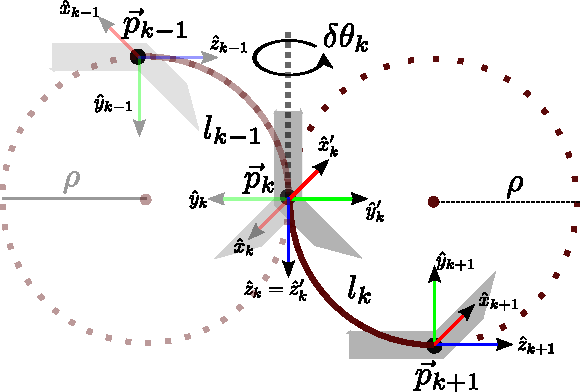
\includegraphics[scale=0.9]{Figures/NeedleKinematics.pdf}
\caption{Needle Kinematics}
\label{fig_nk}
\end{figure}

In this work, the state estimation problem for steerable needles is formulated in the Bayesian Filtering framework described in \cite{Thrun:2005}.
\begin{align}  \label{eqn:stateest}
&\underbrace{\stateest}_{\text{current state estimate}} = \eta \underbrace{\motion}_{\text{motion model}} \underbrace{\meas}_{\text{measurement model}}
\end{align}
The left side of equation (\ref{eqn:stateest}) is a probability distribution representing the needle's state, $\bvar{x}{k}$.  With certain independence assumptions for the needle's states and measurements \cite{Thrun:2005}, this probability distribution can be decomposed into two distributions. Each component distribution of the state estimate can be computed in an efficient manner:  a motion model describes how the system responds to input $\bvar{u}{k}$, and a measurement model captures the distribution of measurements one would expect given the system's state.   In practice, we implement the Bayesian filtering using a particle filter \cite{Thrun:2005}.


\subsection{Needle Steering State} \label{subsec:state}
Figure \ref{fig_nk} provides a diagram of the unicycle kinematic model for needle steering.  In this model, the state of the system $\bvar{x}{k} =  \left[\vec{p}_k, R_k\right]^\top$ is completely defined by the position of the needle tip, $\vec{p}_k$ and the orientation of a frame attached to the needle tip, $R_k = \left[\hat{x}_k,\hat{y}_k,\hat{z}_k\right] \in \text{SO(3)}$.  In addition to the tip position and orientation,  we augment the unicycle kinematic model state with the $N$ most recent command inputs $\bvar{u}{k-1...k-N}$
\begin{equation*}
\bvar{x}{k} =  \left[\underbrace{\vec{p}_k,}_{\text{tip position}} \underbrace{R_k,}_{\text{tip orienation}} \underbrace{\bvar{u}{k-1,...,k-N}}_{\text{previous commands}}\right]^\top
\end{equation*}
These command inputs are described in section \ref{subsec:unicycle} below.


\subsection{Motion Model} \label{subsec:unicycle}
In this work, we use the unicycle kinematic model proposed in \cite{Park2005}.  This model has previously been used and validated for closed loop control of steerable needles in \cite{Majewicz2013} and \cite{adebar2014recursive}.  In the unicycle kinematic model, steerable needles are assumed to naturally follow circular paths of constant curvature in a plane determined by the orientation and position of the needle's tip.  Control of the needle is achieved through two degrees of freedom, insertion and rotation of the needle about its axis.

In \cite{adebar2014recursive}, a stochastic state update equation,
\begin{equation*}
\bvar{x}{k+1} = f(\bvar{x}{k}, \bvar{u}{k}, \bvar{w}{k})
\end{equation*}  
was described for the unicycle kinematic model, where $\bvar{x}{k+1}$ is the needle's state at time-step $k+1$. $\bvar{u}{k}$ and $\bvar{w}{k}$ are the control and disturbance vectors at time $k$ and are described below.  

At each time-step, the needle is rotated about its axis by $\delta \theta_k$ and inserted a distance $l_k$.  These actions define the control input 
\begin{equation*}
\bvar{u}{k} = \left[l_k, \delta\theta_k\right]^\top
\end{equation*}  

During an insertion, the unicycle kinematic model assumes the needle will travel along a circular arc.  The radius of curvature of this arc, $\rho$, is assumed to be constant and is governed by the stiffness of both the tissue and needle.  

A state update is first calculated assuming no process noise, producing a new ideal state, $\bvar{x}{k+1}^{\text{ideal}} = \left[\vec{p}^{\text{ideal}}_{k+1}, R^{\text{ideal}}_{k+1}\right]$.  This is done by rotating the coordinate frame attached to the needle tip, $R_k$, about $\hat{z}_k$ by $\delta \theta$ radians to yield an intermediate frame $R' = [\hat{x}', \hat{y}', \hat{z}']$:
\begin{equation*}
R' = R_{\hat{z}_k}(\delta\theta)R_k
\end{equation*}
In the plane defined by intermediate tip frame axes $\hat{y}'_k$ and $\hat{z}'_k$, the tip position is moved along a $\frac{l_k}{\rho}$ radian arc segment of length $l_k$ to yield a new tip position, $\vec{p}^{\text{ideal}}_{k+1}$.  Finally, $R'$ is rotated by $\frac{\l_k}{\rho}$ radians about $\hat{x}'$ to yield an updated coordinate frame
\begin{equation*}
R^{\text{ideal}}_{k+1} = [\hat{x}^{\text{ideal}}_k, \hat{y}^{\text{ideal}}_k, \hat{z}^{\text{ideal}}_k] = R_{\hat{x}'_k}\left(\frac{l_k}{\rho}\right)R'
\end{equation*}
so that $\hat{z}^{\text{ideal}}_{k+1}$ is tangent with the ideal needle's trajectory at time $k+1$.  

The ideal needle state update described above has error from both inaccuracies in the kinematic model as well as disturbances such as tissue in-homogeneity, vasculature, and tissue fascia.  Because of this, the ideal unicycle kinematic model was modified in \cite{adebar2014recursive} to account for error in both position and orientation.  These errors are captured in the process noise random variable 
\begin{equation*}
\bvar{w} = \left[\vec{w}_{p_k}, W_{R_k}\right]
\end{equation*}  
which has a position noise component, $\vec{w}_{p_k}$ and an orientation noise component, $W_{R_k}$.  $\vec{w}_{p_k}$ is added to $\vec{p}^{\text{ideal}}_{k+1}$ to yield the final position $\vec{p}_{k+1}$.
Similarly, the orientation noise component perturbs $R^{ideal}_{k+1}$ to yield the final orientation $R_{k+1}$
\begin{align*}
\vec{p}_{k+1} &= \vec{p}^{\text{ideal}}_{k+1}+\vec{w}_{p_k} \\
R_{k+1} &= W_{R_k}R^{\text{ideal}}_{k+1}
\end{align*}
With the stochastic state update function, $f$, the probability of being in state $x_k$ can be calculated given a previous state and action.  Therefore the motion model can be calculated as 
\begin{align*}
& p(\bvar{x}{k}|\bvar{x}{k-1},\bvar{u}{k}) = \int_{\bvar{x}{k-1}} p(X_k = \bvar{x}{k} | u_k, \bvar{x}{k-1}) \mathrm{d}\bvar{x}{k-1}
\end{align*}
In practice, the motion model distribution is approximated in the particle filter as the particle propagation step.
\subsection{Measurement Model} \label{subsec:measurement}
In this work, a combination of Doppler and B-mode images from a tracked 2D transducer are used for sensing the steerable needle.  As described in section \ref{sec:imageproc} each image is processed to produce a measurement
\begin{dmath*}
\bvar{z}{k} = \left[\underbrace{x_{\text{im}},y_{\text{im}},}_{\text{image coords.}} \underbrace{d,}_{\text{Doppler response}} \underbrace{\vec{p}_{\text{us}},}_{\text{transducer pos.}} \underbrace{R_{\text{us}}}_{\text{transducer orientation}}\right]^\top
\end{dmath*}

 
\section{Conclusion}
The conclusion goes here.


% use section* for acknowledgement
\section*{Acknowledgment}
The authors would like to thank...


% trigger a \newpage just before the given reference
% number - used to balance the columns on the last page
% adjust value as needed - may need to be readjusted if
% the document is modified later
%\IEEEtriggeratref{8}
% The "triggered" command can be changed if desired:
%\IEEEtriggercmd{\enlargethispage{-5in}}

% references section

% can use a bibliography generated by BibTeX as a .bbl file
% BibTeX documentation can be easily obtained at:
% http://www.ctan.org/tex-archive/biblio/bibtex/contrib/doc/
% The IEEEtran BibTeX style support page is at:
% http://www.michaelshell.org/tex/ieeetran/bibtex/
%\bibliographystyle{IEEEtran}
% argument is your BibTeX string definitions and bibliography database(s)
%\bibliography{IEEEabrv,../bib/paper}
%
% <OR> manually copy in the resultant .bbl file
% set second argument of \begin to the number of references
% (used to reserve space for the reference number labels box)
\bibliographystyle{IEEEtran} 
\bibliography{library}

% biography section
% 
% If you have an EPS/PDF photo (graphicx package needed) extra braces are
% needed around the contents of the optional argument to biography to prevent
% the LaTeX parser from getting confused when it sees the complicated
% \includegraphics command within an optional argument. (You could create
% your own custom macro containing the \includegraphics command to make things
% simpler here.)
%\begin{IEEEbiography}[{\includegraphics[width=1in,height=1.25in,clip,keepaspectratio]{mshell}}]{Michael Shell}
% or if you just want to reserve a space for a photo:

\begin{IEEEbiography}{Michael Shell}
Biography text here.
\end{IEEEbiography}

% if you will not have a photo at all:
\begin{IEEEbiographynophoto}{John Doe}
Biography text here.
\end{IEEEbiographynophoto}

% insert where needed to balance the two columns on the last page with
% biographies
%\newpage

\begin{IEEEbiographynophoto}{Jane Doe}
Biography text here.
\end{IEEEbiographynophoto}

% You can push biographies down or up by placing
% a \vfill before or after them. The appropriate
% use of \vfill depends on what kind of text is
% on the last page and whether or not the columns
% are being equalized.

%\vfill

% Can be used to pull up biographies so that the bottom of the last one
% is flush with the other column.
%\enlargethispage{-5in}



% that's all folks
\end{document}


